% Chapter Template

\chapter{Study Methodology}\doublespacing % Main chapter title

\label{Chapter3} % Change X to a consecutive number; for referencing this chapter elsewhere, use \ref{ChapterX}

\lhead{Chapter III. \emph{Study Methodology}} % Change X to a consecutive number; this is for the header on each page - perhaps a shortened title

%----------------------------------------------------------------------------------------
%	SECTION 1
%----------------------------------------------------------------------------------------
\section{Research Approach}

The research methodology adopted in this study follows an experimental and analytical approach. 
The objective of the study is to analyze malware behavior in Windows operating systems and 
visualize the attack flow using the proposed Malviz framework.

The study focuses on analyzing system level activities such as process creation, API calls, 
system calls, registry modifications, and privilege escalation attempts. The collected data 
is analyzed and transformed into graphical visualizations to help security analysts understand 
malware behavior more effectively.

The methodology involves both static and dynamic malware analysis techniques in a controlled 
environment.


\section{Experimental Environment}

To safely analyze malware behavior, a controlled virtual environment was created. 
The experiments were conducted using virtualization to isolate the system from 
the host machine.

\begin{table}[H]
\centering
\begin{tabular}{|c|c|}
\hline
Component & Description \\
\hline
Target System & Windows 10 Virtual Machine \\
Attack Machine & Kali Linux \\
Virtualization Platform & VirtualBox \\
Monitoring Tools & Process Monitor, Wireshark \\
Reverse Engineering Tools & Ghidra, x64dbg \\
Privilege Analysis Tools & SharpUp \\
Password Cracking Tool & Hashcat \\
\hline
\end{tabular}
\caption{Experimental Environment Setup}
\end{table}

\section{Data Collection}

During malware execution, several system level activities were monitored and recorded. 
The following types of data were collected for analysis:

\begin{itemize}
\item Process creation events
\item System call activity
\item File system modifications
\item Registry changes
\item Network communication
\item Privilege escalation attempts
\end{itemize}

The collected behavioral data was used as input for the Malviz visualization system.

\section{Malware Analysis Process}

Malware samples were analyzed using both static and dynamic analysis techniques.

\textbf{Static Analysis:}

Static analysis involves examining the malware executable without executing it. 
Tools such as PEStudio and Ghidra were used to inspect the Portable Executable (PE) 
structure, imported libraries, and embedded strings.

\textbf{Dynamic Analysis:}

Dynamic analysis involves executing malware inside an isolated virtual machine while 
monitoring its runtime behavior. Tools such as Process Monitor and Wireshark were used 
to observe system calls, registry modifications, and network activity.

\section{Privilege Escalation Analysis}

Privilege escalation techniques were studied to understand how attackers gain higher 
privileges within the Windows operating system.

The study focused on analyzing password hashes stored in the Security Account Manager (SAM) database.

The SAM file is located at:

\begin{verbatim}
C:\Windows\System32\config\SAM
\end{verbatim}

The following steps were used during privilege escalation experiments:

\begin{enumerate}
\item Gain initial access to the system
\item Extract SAM and SYSTEM registry files
\item Extract password hashes using secretsdump
\item Crack NTLM hashes using Hashcat
\item Obtain administrator credentials
\end{enumerate}

Example command used to extract password hashes:

\begin{verbatim}
secretsdump.py -sam SAM -system SYSTEM local
\end{verbatim}

\section{System Call Analysis using Hell's Gate}

Modern malware often bypasses traditional API monitoring by invoking system calls directly. 
To understand this technique, the Hell's Gate method was studied.

The Hell's Gate technique dynamically retrieves system call numbers from the NTDLL module 
instead of relying on static API functions.

The methodology for resolving system calls involves:

\begin{enumerate}
\item Accessing the Process Environment Block (PEB)
\item Locating the NTDLL module in memory
\item Traversing the Export Address Table
\item Extracting system call numbers dynamically
\end{enumerate}

Example instruction pattern used by NTDLL system calls:

\begin{verbatim}
mov r10, rcx
mov eax, syscall_number
syscall
ret
\end{verbatim}

This technique allows malware to execute system calls directly, bypassing API monitoring 
mechanisms used by security tools.

\section{Malviz Visualization Framework}

The Malviz framework was developed to visualize malware behavior in an interactive manner. 
The system collects runtime behavioral data and converts it into graphical representations.

The visualization module helps analysts identify suspicious behavior patterns by presenting 
system activity in a structured and intuitive format.

The system generates the following types of visualizations:

\begin{itemize}
\item Process interaction graphs
\item System call flow diagrams
\item Privilege escalation timelines
\end{itemize}

\subsection{Malware Analysis Workflow}

\begin{figure}[H]
\centering
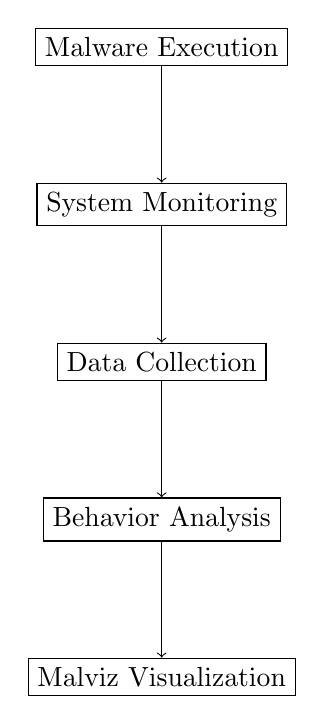
\begin{tikzpicture}[node distance=2cm]

\node (malware) [rectangle, draw] {Malware Execution};
\node (monitor) [rectangle, draw, below of=malware] {System Monitoring};
\node (collect) [rectangle, draw, below of=monitor] {Data Collection};
\node (analysis) [rectangle, draw, below of=collect] {Behavior Analysis};
\node (visual) [rectangle, draw, below of=analysis] {Malviz Visualization};

\draw[->] (malware) -- (monitor);
\draw[->] (monitor) -- (collect);
\draw[->] (collect) -- (analysis);
\draw[->] (analysis) -- (visual);

\end{tikzpicture}
\caption{Malviz Malware Analysis Workflow}
\end{figure}

\section{Evaluation}

The proposed system was evaluated by executing malware samples within the controlled 
virtual environment and observing their behavioral patterns. The collected data was 
visualized using the Malviz framework to analyze how malware interacts with system 
resources and attempts privilege escalation.

The effectiveness of the system was evaluated based on its ability to clearly represent 
malware behavior and assist in identifying suspicious activities.
\section{Summary}

This chapter described the methodology adopted to analyze malware behavior and 
study privilege escalation techniques within Windows operating systems. 
A controlled virtual environment was established to safely execute and monitor 
malware samples. Both static and dynamic malware analysis techniques were used 
to examine executable structures, system calls, registry modifications, and 
network activity.

The study also explored common privilege escalation mechanisms such as SAM 
hash extraction and password cracking using tools like \texttt{secretsdump} 
and \texttt{Hashcat}. In addition, modern system call evasion techniques such 
as the Hell's Gate method were analyzed to understand how malware dynamically 
retrieves and executes system calls directly from \texttt{NTDLL.dll}, thereby 
bypassing traditional API monitoring mechanisms.

The collected behavioral data was then processed and visualized using the 
proposed \textbf{Malviz} framework. This visualization approach helps security 
analysts interpret complex malware activities more effectively by presenting 
system interactions, process behavior, and privilege escalation attempts in 
a structured graphical format. The methodology presented in this chapter forms 
the foundation for the implementation and evaluation of the Malviz system 
discussed in the following chapters.

